\documentclass[preprint,11pt]{elsarticle}
%DIF LATEXDIFF DIFFERENCE FILE
%DIF DEL tmp\v38_flat.tex   Thu Nov 26 01:32:49 2026
%DIF ADD tmp\v39_flat.tex   Thu Nov 26 01:35:30 2026

\usepackage{amsmath,amssymb}
\usepackage{booktabs}
\usepackage{graphicx}
\usepackage{float}
\usepackage{hyperref}
\usepackage{xcolor}
\usepackage{siunitx}
\usepackage{seqsplit}
\usepackage[a4paper,margin=2.4cm]{geometry}

\graphicspath{{figures/}}
\hypersetup{
  hidelinks,
  pdftitle={Fusion Utility Depends on the Evaluator: A Boundary Study of Confidence-Shielded Input Selection for Infrared-Visible Object Detection},
  pdfauthor={Jianyong Zhao, Zigao Wu, Mengfei Ma},
  pdfsubject={Research paper submitted to Infrared Physics \& Technology},
  pdfkeywords={infrared-visible image fusion, object detection, fusion-input selection, confidence-gated fallback, selective prediction, thermal imaging}
}

\journal{Infrared Physics \& Technology}
\biboptions{numbers,sort&compress}
%DIF PREAMBLE EXTENSION ADDED BY LATEXDIFF
%DIF CFONT PREAMBLE %DIF PREAMBLE
\RequirePackage{color}\definecolor{RED}{rgb}{1,0,0}\definecolor{BLUE}{rgb}{0,0,1} %DIF PREAMBLE
\DeclareOldFontCommand{\sf}{\normalfont\sffamily}{\mathsf} %DIF PREAMBLE
\providecommand{\DIFaddtex}[1]{{\protect\color{blue} \sf #1}} %DIF PREAMBLE
\providecommand{\DIFdeltex}[1]{{\protect\color{red} \scriptsize #1}} %DIF PREAMBLE
%DIF SAFE PREAMBLE %DIF PREAMBLE
\providecommand{\DIFaddbegin}{} %DIF PREAMBLE
\providecommand{\DIFaddend}{} %DIF PREAMBLE
\providecommand{\DIFdelbegin}{} %DIF PREAMBLE
\providecommand{\DIFdelend}{} %DIF PREAMBLE
\providecommand{\DIFmodbegin}{} %DIF PREAMBLE
\providecommand{\DIFmodend}{} %DIF PREAMBLE
%DIF FLOATSAFE PREAMBLE %DIF PREAMBLE
\providecommand{\DIFaddFL}[1]{\DIFadd{#1}} %DIF PREAMBLE
\providecommand{\DIFdelFL}[1]{\DIFdel{#1}} %DIF PREAMBLE
\providecommand{\DIFaddbeginFL}{} %DIF PREAMBLE
\providecommand{\DIFaddendFL}{} %DIF PREAMBLE
\providecommand{\DIFdelbeginFL}{} %DIF PREAMBLE
\providecommand{\DIFdelendFL}{} %DIF PREAMBLE
%DIF HYPERREF PREAMBLE %DIF PREAMBLE
\providecommand{\DIFadd}[1]{\texorpdfstring{\DIFaddtex{#1}}{#1}} %DIF PREAMBLE
\providecommand{\DIFdel}[1]{\texorpdfstring{\DIFdeltex{#1}}{}} %DIF PREAMBLE
%DIF COLORLISTINGS PREAMBLE %DIF PREAMBLE
\RequirePackage{listings} %DIF PREAMBLE
\RequirePackage{color} %DIF PREAMBLE
\lstdefinelanguage{DIFcode}{ %DIF PREAMBLE
%DIF DIFCODE_CFONT %DIF PREAMBLE
  moredelim=[il][\color{red}\scriptsize]{\%DIF\ <\ }, %DIF PREAMBLE
  moredelim=[il][\color{blue}\sffamily]{\%DIF\ >\ } %DIF PREAMBLE
} %DIF PREAMBLE
\lstdefinestyle{DIFverbatimstyle}{ %DIF PREAMBLE
	language=DIFcode, %DIF PREAMBLE
	basicstyle=\ttfamily, %DIF PREAMBLE
	columns=fullflexible, %DIF PREAMBLE
	keepspaces=true %DIF PREAMBLE
} %DIF PREAMBLE
\lstnewenvironment{DIFverbatim}[1][]{\lstset{style=DIFverbatimstyle}}{} %DIF PREAMBLE
\lstnewenvironment{DIFverbatim*}[1][]{\lstset{style=DIFverbatimstyle,showspaces=true}}{} %DIF PREAMBLE
\lstset{extendedchars=\true,inputencoding=utf8}

%DIF END PREAMBLE EXTENSION ADDED BY LATEXDIFF

\begin{document}
\sloppy

\begin{frontmatter}

\title{Fusion Utility Depends on the Evaluator: A Boundary Study of Confidence-Shielded Input Selection for Infrared--Visible Object Detection}

\author[AUTHOR]{Jianyong Zhao}
\ead{shaohaojia2001@163.com}
\ead[url]{https://orcid.org/0009-0005-3251-2785}

\author[AUTHOR]{Zigao Wu\corref{cor1}}
\ead{zgwu@ncepu.edu.cn}
\ead[url]{https://orcid.org/0000-0002-7449-343X}

\author[AUTHOR]{Mengfei Ma}
\ead{MYmmf01@163.com}
\ead[url]{https://orcid.org/0009-0007-1328-1314}

\cortext[cor1]{Corresponding author.}
\affiliation[AUTHOR]{organization={North China Electric Power University},
            addressline={Hebei},
            city={Baoding},
            postcode={071003},
            country={China}}

\begin{abstract}
Infrared and visible fusion can expose complementary evidence, but the same
fused image may improve one detector and degrade another. We evaluate
Confidence-Shielded, Evaluator-Conditioned Fusion-Input Selection (CS-ECF),
which scores visible input, consensus-detail fusion (CDF), PIAFusion, and
SPGFusion using the mean of the five highest target-detector confidences. A
fused input is selected only when its score reaches 1.5 times the visible
score; otherwise visible input is retained. Ground truth is not used at
inference.

On scene-disjoint LLVIP, the visible-input contrast was \(+0.00012\)
\([-0.00484,+0.00670]\), and CS-ECF did not outperform Always CDF. Relative to
no-shield selection it gained \(+0.00894\) \([+0.00096,+0.02155]\), exceeding
a switch-matched random control by \(+0.01392\)
\([+0.00964,+0.02023]\). \DIFdelbegin \DIFdel{The }\DIFdelend \DIFaddbegin \DIFadd{For the four-candidate policy, the }\DIFaddend AP50--95 benefit
did not persist. VEDAI also favoured the shield over no shield by \(+0.0410\),
although visible remained better by \(0.0136\). External evaluators reversed
both orderings.

With score depth and margin fixed, a development-set candidate-library
selection chose visible plus PIAFusion. \DIFdelbegin \DIFdel{This }\DIFdelend \DIFaddbegin \DIFadd{On a later 900-frame LLVIP holdout, this
}\DIFaddend two-candidate policy \DIFdelbegin \DIFdel{used two
rather than four detector passes and gained \(+0.00337\)
\([-0.00016,+0.01267]\) }\DIFdelend \DIFaddbegin \DIFadd{gained \(+0.01560\) \([+0.00249,+0.02874]\) }\DIFaddend AP50 \DIFdelbegin \DIFdel{over visible }\DIFdelend and
\DIFdelbegin \DIFdel{\(+0.01218\)
\([+0.00136,+0.02915]\) over no shield on LLVIP. It }\DIFdelend \DIFaddbegin \DIFadd{\(+0.00946\) \([+0.00113,+0.01769]\) AP50--95 over visible input, with positive
gains in all three sequences and six checkpoints. Ungated PIAFusion reversed
strongly on one sequence. The policy }\DIFaddend did not transfer to VEDAI or independent
DroneVehicle runs. \DIFaddbegin \DIFadd{A measured end-to-end pipeline median was \(1.67\) s versus
\(2.52\) s for the full library, still above real time. }\DIFaddend CS-ECF is therefore
supported only as a checkpoint- and domain-specific AP50 safeguard after
independent validation.
\DIFdelbegin \DIFdel{It is not a general accuracy gain, localization-robust safeguard, risk
guarantee, or low-latency deployment method.
}\DIFdelend \end{abstract}

\begin{keyword}
infrared--visible image fusion \sep object detection \sep
evaluator-conditioned fusion-input selection \sep confidence-gated fallback \sep
selective prediction \sep thermal imaging
\end{keyword}

\end{frontmatter}

\section{Introduction}

Visible and infrared imaging provide complementary evidence. Visible cameras
capture fine spatial detail and color, whereas infrared sensors can retain
target contrast under poor illumination or smoke. These properties have
motivated pixel-, feature-, and network-based fusion methods for surveillance,
autonomous perception, and thermal imaging systems
\cite{ma2019survey,mudavath2026review,zhu2017tophat,zhang2020,ma2019fusiongan,li2019densefuse,xu2022u2fusion,li2021rfn,yi2024diffif,yang2025lfdt}.
For object detection, however, the value of a fused image depends on more than
visual appeal. It is defined by the change in detector outputs under a
specified operating condition.

Many benchmark-oriented fusion studies select one fused representation and
evaluate it with one detector on one benchmark. This reporting choice is
appropriate for a fixed deployed detector. The present study addresses a
different setting in which the detector checkpoint or operating domain may
change. Detectors differ in receptive-field size, confidence calibration,
training data, and sensitivity to high-frequency detail
\cite{abdar2021uncertainty,gawlikowski2023uncertainty}. A fusion rule that
improves one evaluator may therefore reduce the average precision (AP) of
another on the same image.

Per-image selection offers a natural response: evaluate several fusion
candidates and choose the one with the strongest detector response.
Unconstrained selection, however, can turn small calibration differences into
frequent input switches and severe AP losses when a spurious high-confidence
response is mistaken for better detection. The task is therefore to decide
when the evidence is strong enough to depart from the visible-image fallback,
which is related to the classical reject option in recognition
\cite{chow1970reject}.

Recent infrared--visible fusion and detection studies have optimized shared
fusion networks, cross-modal feature fusion, or hierarchical detectors
\cite{zhao2025cmifdf,gao2026coifsd,an2026mrtdetr,zhang2026hffn,wan2025yolo11rgbt}.
General-purpose detectors provide the evaluator side of this problem
\cite{redmon2016yolo,zhao2024rtdetr}. These studies show why fusion and
detection should be considered jointly, but they generally train or optimize a
detector--fusion system. We therefore ask whether a simple confidence-gated
choice among already generated inputs can reduce detector-specific sensitivity,
and we report where that choice fails.

We formulate infrared--visible fusion selection as evaluator-conditioned input
arbitration. CS-ECF evaluates four candidates with the target detector,
computes a top-five confidence score, and accepts a fused candidate only when
its score reaches 1.5 times that of the visible input. The margin was selected
on development data and then held unchanged on new LLVIP scenes. Our question
is deliberately narrower than whether the gate is a generally superior
fusion-selection method. We address three questions. First, how much do fixed
candidate rankings change across detector checkpoints and domains? Second, does
the confidence margin reduce switching loss beyond a matched switch frequency,
and does it improve on visible or fixed CDF? Third, after validation, is the
four-candidate library necessary? The contributions are:
\begin{enumerate}
  \item a budgeted candidate-library procedure that holds the confidence score
  and margin fixed while selecting the smallest development-feasible input
  library, together with its held-out and cross-domain boundaries;
  \item a candidate-by-checkpoint analysis showing fixed fusion, no-shield
  selection, and CS-ECF changing order across evaluators;
  \item a scene-disjoint LLVIP evaluation with standard confidence-ordered
  AP matching, a prespecified local primary visible-input contrast, and a
  switch-budget-matched random control;
  \item separate DroneVehicle and VEDAI tests plus a same-split single-seed
  YOLOv11-RGBT implementation pilot, reported with explicit mechanism,
  portability, localization, and optimization boundaries.
\end{enumerate}

\section{Related work}

\subsection{Fusion representations}

Classical infrared--visible fusion methods combine complementary evidence using
handcrafted transforms or representations. Representative examples include
multi-scale top-hat transforms, non-subsampled contourlet transforms with
compressed sensing, two-scale saliency decomposition, and three-scale framelet
or shear representations \cite{zhu2017tophat,zhang2016nsct,zhang2021twoscale,wei2017threescale}.
Sparse-representation methods instead describe local image content with learned
or overcomplete dictionaries before applying a coefficient-level fusion rule
\cite{yin2013sparsefusion,yin2015multiscale}. These methods explicitly preserve
target contrast, edges, and local saliency. Their fusion rules are typically
designed for image-level visual quality rather than for the ranking assigned by
a particular detector.

Learned fusion models replace handcrafted combination rules with trainable
feature extraction and reconstruction. DenseFuse, IFCNN, U2Fusion, and RFN-Nest
are representative encoder--decoder or residual designs
\cite{li2019densefuse,zhang2020,xu2022u2fusion,li2021rfn}. Adversarial
formulations add discriminative losses for texture and target preservation
\cite{ma2019fusiongan,hou2021ssgan,yi2021dfpgan,song2022tdgan}.
Wavelet-based dual-path networks and transformer-based designs have since added
multi-scale context and long-range interaction
\cite{liu2023dualpath,hao2022vdfefuse,yang2023dglt,an2024mras}, while diffusion
models introduced generative priors for fusion \cite{yi2024diffif,yang2025lfdt}.
These methods broaden the candidate design space but generally produce a single
fused output. They do not specify how to select among several available
candidates for a fixed deployed detector.

\subsection{Task-aware fusion and detection}

Task-aware fusion introduces an illumination, semantic, or saliency signal into
the transfer rule. PIAFusion conditions fusion on illumination
\cite{tang2022}; SPGFusion and MTFusion incorporate semantic priors
\cite{zhang2026,zhou2026mtfusion}; and classification-saliency or masked
autoencoder designs use auxiliary representations to decide which features to
retain \cite{xu2021classsaliency,wang2025smae}. Such priors make the transfer
more selective, but a proxy such as illumination or segmentation does not
guarantee a better confidence ordering for every detector.

One-stage and DETR-style detectors exhibit different confidence behavior and
receptive-field structure \cite{redmon2016yolo,wang2024yolov9,wang2024yolov10,zhao2024rtdetr}.
Recent infrared--visible systems have integrated fusion with detection through shared
backbones, cross-modal feature exchange, saliency masking, or hierarchical
fusion \cite{zhao2025cmifdf,gao2026coifsd,an2026mrtdetr,zhang2026hffn,wan2025yolo11rgbt,xiang2025unifusod,yue2022lowlight}.
YOLOv11-RGBT provides a comprehensive single-stage framework that can omit or
combine cross-modal features at different network depths. The cited version is
a 2025 preprint implementation, and the present paper evaluates one fixed
training recipe rather than the attainable performance of the framework. These
systems optimize detection and representation together, but they do not specify
an inference-time rule for arbitrating among already generated candidate inputs.
Joint optimization aligns the fused representation with the detector, but the
learned coupling is specific to a training objective. It does not itself
provide an inference-time rule, free of ground-truth boxes, for choosing among generated
fusion candidates when the target checkpoint or data composition changes.

\subsection{Evaluation and selection boundary}

Fusion quality has commonly been assessed with reference or no-reference image
metrics \cite{ma2019survey,mudavath2026review}. Those scores summarise source
retention or perceptual quality; they do not identify which of several inputs
will produce the higher AP for a particular detector. Multispectral
detection studies show that thermal evidence can improve robustness under
poor illumination \cite{li2010thermal,guo2024prior}, but gains depend on
architecture, training data, and the operating regime
\cite{abdar2021uncertainty,gawlikowski2023uncertainty}. The same dependence appears
visible across the detector checkpoints examined here.

The decision to depart from a visible-image fallback resembles the classical
reject option \cite{chow1970reject}, but the object of the decision is an input
candidate rather than a class prediction. The threshold must therefore be
specified independently of test-set performance, fixed before held-out
evaluation, and
evaluated against both mean gain and observed tail loss. This study evaluates a
simple confidence gate rather than claiming a new selective-prediction theory.
We report whether the gate improves on visible and on the strongest fixed input
under matched evaluation, and where the observed trade-off does not reproduce.

\subsection{Positioning}

CS-ECF does not introduce another image-fusion operator. It treats an existing
fusion library as a set of alternative inputs and uses the target detector as
an evaluator that requires no ground-truth boxes during inference. Unlike
task-aware networks, it requires neither a new fusion model nor joint
detector--fusion training. Unlike fixed image-quality rankings, it measures
detector utility directly while accounting for checkpoints and scene or frame
groups. The contribution is an empirical arbitration study and boundary
analysis, not a demonstrated replacement for a fixed fused input. We do not
claim a new general routing theory, and a direct comparison with learned
per-image routing or selective object-detection policies remains outside the
present evidence boundary.

\section{Methods}

Throughout, a fusion input is one candidate image supplied to a detector, an
evaluator is the target detector checkpoint used to score that image, and a
training run is one fitted model trajectory. Two checkpoints from one training
run are not independent. An evaluation group is a scene, frame group, or
consecutive frame block within which detections are not treated as independent
runs.

\subsection{Problem formulation}

We denote a registered visible--infrared pair by \(x_v\) and \(x_i\), and the
target detector checkpoint by \(\mathcal{D}\). A candidate
\(c\in\mathcal{C}\) produces an input image \(x_c\), where
\(\mathcal{C}=\{\mathrm{vis},\mathrm{cdf},\mathrm{pia},\mathrm{spg}\}\).
The policy returns one candidate per pair without access to ground-truth boxes:
\begin{equation}
g(x_v,x_i;\mathcal{D})\in\mathcal{C}.
\end{equation}
The final detection output is
\(\mathcal{D}(x_{g(x_v,x_i;\mathcal{D})})\). Because the same detector is used
to evaluate candidates and to produce final detections, the policy requires no
separate test-time ground-truth predictor.

\subsection{Fusion candidates}

The visible input is always retained as a fallback candidate. CDF is a
study-internal candidate constructed for this comparison; it is not a
previously published fusion operator. It combines a pixel-mean image and an
IFCNN image using sign-consistent high-frequency details. We denote the
pixel-mean and IFCNN images by \(x_m\) and \(x_f\),
respectively, and let \(G_\sigma\) denote Gaussian blur with \(\sigma=5\). The
corresponding detail images are
\(d_m=x_m-G_\sigma*x_m\) and \(d_i=x_f-G_\sigma*x_f\). Their consensus detail
is
\begin{equation}
d(x)=
\begin{cases}
\operatorname{sign}(d_m+d_i)\min(|d_m|,|d_i|), & d_m d_i>0,\\
0, & \text{otherwise}.
\end{cases}
\end{equation}
A thermal-validity mask \(M\) combines the infrared top-hat response, infrared
intensity, visible luminance, connected components, and spatial smoothing. The
quantile \(q_{\mathrm{TH}}=0.95\) marks the top-hat response above which a pixel
is considered thermally salient. This quantity differs from the candidate score
\(q_c\) defined below. We applied a \(31\times31\) elliptical top-hat kernel and
an infrared floor of 120. Candidate regions also required a visible-luminance
cutoff at the 75th percentile, \(5\times5\) morphological opening, and connected
components of at least 64 pixels. The surviving mask was then dilated and
smoothed with \(31\times31\) kernels. Shared detail was injected into the LAB
luminance channel as
\begin{equation}
L' = L + \alpha M d.
\end{equation}
The frozen settings are \(q_{\mathrm{TH}}=0.95\), \(\alpha=0.20\), and
\(\sigma=5\). These are engineering defaults for the study-internal CDF
candidate, not parameters selected to optimize a published fusion method.
The Supplementary Material reports one-at-a-time sensitivity to
\(q_{\mathrm{TH}}\), \(\alpha\), \(\sigma\), and the minimum consensus-detail
magnitude. PIAFusion and SPGFusion were generated using their
official model definitions and pretrained weights under the same image-pair protocol
\cite{zhang2020,tang2022,zhang2026}.

\subsection{Confidence-shielded arbitration}

For candidate \(c\), let \(s_{c,1}\ge s_{c,2}\ge\cdots\) denote detector
confidences sorted in descending order. We define the candidate score as
\begin{equation}
q_c=\frac{1}{\min(K,n_c)}
\sum_{j=1}^{\min(K,n_c)}s_{c,j},
\qquad K=5,
\end{equation}
where \(n_c\) is the number of detections. Candidates with no detections receive
\(q_c=-1\). The highest-scoring candidate is
\(c^\ast=\arg\max_c q_c\), with ties broken in favor of visible. The selected
input is
\begin{equation}
c=
\begin{cases}
c^\ast, & c^\ast\ne\mathrm{vis}\ \text{and}\ q_{c^\ast}\ge1.5q_{\mathrm{vis}},\\
\mathrm{vis}, & \text{otherwise}.
\end{cases}
\end{equation}
The complete inference path, including visible fallback, is shown in
Fig.~\ref{fig:workflow}. The top-five mean reduces reliance on a single
detection while excluding the low-confidence tail. The candidate set includes
the visible fallback and representative region-selected, learned, and published
fusion methods. The policy is ground-truth-box-free at inference.

The value \(q_c=-1\) is an explicit no-detection sentinel rather than a
measured confidence. In the retrospective 12-checkpoint matrix it occurred for
visible input in 1 of 3,400 image-checkpoint cases and not in the 8,370
image-checkpoint cases of the primary LLVIP holdout. The single retrospective
case switched to PIAFusion and improved per-image AP50 from 0 to 0.505. We did
not add an absolute confidence floor in the frozen policy because all primary
held-out inputs contained visible detections and the only observed sentinel
case was beneficial. A floor therefore has no estimable effect in the primary
data; it is reported as an unresolved low-prevalence boundary rather than as
validated protection.

The margin was originally selected on 150 LLVIP and 400 M3FD development
images using two detectors per dataset. The LLVIP development and training
frames had no stem overlap but came from the same scene-source group. This
split was therefore image-disjoint, but not scene-group-disjoint, and the
available search records lacked an external timestamp. These limitations
prevent treating the original multi-dataset analysis as independent
validation.

We therefore recorded a prospective LLVIP protocol and SHA-256 manifest before
candidate scoring on sequences 040--070. The protocol was not externally
registered. Sequence 040 was restricted to a policy audit, while sequences 050,
060, and 070 were untouched held-out data. The four-candidate library,
top-five score, and 1.5 margin were fixed unchanged. Under the original
selection rule, the audit would have selected 2.0 rather than 1.5; we retained
1.5 because changing the margin after the audit would create a new selection
round. Supplementary Fig.~S8 reports the original development sensitivity
analysis, and the complete development and held-out records appear in the
Supplementary Material.

\begin{figure}[t]
\centering
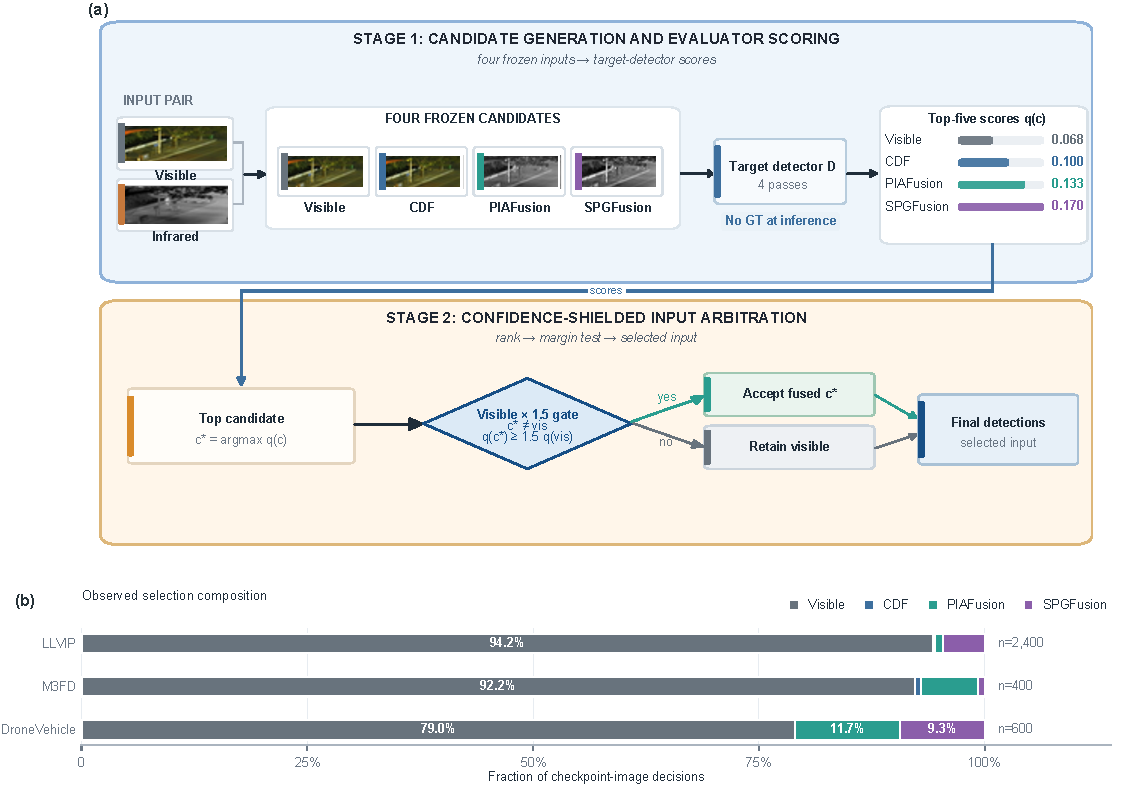
\includegraphics[width=\linewidth]{Figure1_workflow.pdf}
\caption{\textbf{Four-candidate confidence-shielded reference inference.}
(\textbf{a}), Stage 1 constructs four frozen reference candidates from the registered
visible--infrared pair. The target detector scores each candidate by its
top-five confidence without per-image ground truth. Stage 2 ranks the scores
and accepts the highest-scoring fused input \(c^\ast\) only when
\(c^\ast\ne\mathrm{vis}\) and \(q_{c^\ast}\ge1.5q_{\mathrm{vis}}\); otherwise,
visible input is retained. The example uses LLVIP frame 070142 and YOLO26n
seed 0, for which \(q_{\mathrm{SPG}}=0.170\) exceeds the threshold
\(1.5q_{\mathrm{vis}}=0.102\). (\textbf{b}), Composition of the frozen input
decisions in the retrospective 12-checkpoint analysis for LLVIP
(8\(\times\)300), M3FD (2\(\times\)200), and the DroneVehicle official test
subset (2\(\times\)300). Source data are provided in
\texttt{Figure1\_source.csv} and \texttt{Figure1\_example\_scores.csv}.}
\label{fig:workflow}
\end{figure}

For each candidate score depth and margin, we computed the balanced mean gain
and the worst gain over the four development evaluator cells. A setting was
admissible only when every evaluator gain was at least \(-0.0005\) AP50.
Among admissible settings, the frozen rule selected the largest balanced mean;
margin \(1.5\) was frozen before held-out scoring. The competing margins at
\(K=5\) illustrate the choice: margin 1.3 gave a mean of \(+0.0000\) and a worst
gain of \(-0.0026\); margin 1.5 gave \(+0.0008\) and \(-0.0001\); and margin 2.0
gave \(+0.0001\) and \(-0.0004\). Neither \(K\) nor the margin was tuned on
DroneVehicle. The complete selection grid, threshold sensitivity, and
post-freeze score-depth analysis are provided in Supplementary Fig.~S8 because
they are development diagnostics, not held-out evidence.

\subsection{Budgeted candidate-library selection}

We evaluated all eight non-empty subsets of
\(\{\mathrm{vis},\mathrm{CDF},\mathrm{PIAFusion},\mathrm{SPGFusion}\}\) that
contain visible. The score depth and margin were kept at the previously frozen
values \(K=5\) and \(1.5\); this analysis did not perform a second margin
search. For each subset, candidate scores were recomputed on the same four
development evaluator cells used for margin selection, comprising two LLVIP
and two M3FD detectors.

A subset \(S\) was feasible when every development evaluator gain satisfied
\begin{equation}
\Delta \mathrm{AP50}^{\mathrm{dev}}_e(S) \ge -0.0005.
\end{equation}
Let \(\mu(S)\) be the mean of
\(\Delta \mathrm{AP50}^{\mathrm{dev}}_e(S)\) over the four evaluator cells,
\(n(S)\) the number of detector forwards, and \(C(S)\) the measured component
cost. The selected subset was
\begin{equation}
\begin{aligned}
S^\ast&=\arg\operatorname{lexmin}_{S\in\mathcal{F}}
\bigl(n(S),C(S)\bigr),\\
\mathcal{F}&=\left\{S:
\min_e\Delta \mathrm{AP50}^{\mathrm{dev}}_e(S)\ge-0.0005,
\ \mu(S)\ge\mu_{\max}-10^{-5}
\right\}.
\end{aligned}
\end{equation}
This deterministic tie breaking prevents a negligible validation difference
from retaining an expensive candidate. If no fused subset is feasible, the
procedure returns visible input.

The procedure was fixed before the candidate subset was evaluated on the
standard-matched LLVIP \DIFdelbegin \DIFdel{holdout }\DIFdelend \DIFaddbegin \DIFadd{050--070 score archive }\DIFaddend and the external datasets. \DIFdelbegin \DIFdel{The new }\DIFdelend \DIFaddbegin \DIFadd{Those
evaluations were exploratory because the }\DIFaddend subset was not \DIFdelbegin \DIFdel{part of the original
prospective protocol}\DIFdelend \DIFaddbegin \DIFadd{named in the original
protocol. Before scoring a later confirmation set, we recorded a new protocol
and a local SHA-256 sidecar for LLVIP sequences 080}\DIFaddend , \DIFdelbegin \DIFdel{so its held-out evaluation is
reported as exploratory rather than confirmatory. Complete validation and
retrospective grids, raw source data}\DIFdelend \DIFaddbegin \DIFadd{090, and 100. A resource
amendment, also recorded before candidate generation or detector scoring,
fixed the first 300 lexicographically selected non-empty frames in each
sequence. Complete grids}\DIFaddend , \DIFaddbegin \DIFadd{protocols, source hashes, }\DIFaddend and the selection
implementation are provided in the Supplementary Material and analysis
archive.

\subsection{Datasets and evaluators}

The official LLVIP partitions are larger than the subsets used here
\cite{jia2021}. We uniformly shuffled the official test pairs with non-empty
labels using seed 0 and used the first 300 as the test subset. The release
contains 3,463 test pairs with non-empty labels, so 3,163 eligible pairs were
not evaluated. From the official training partition, we selected the
lexicographically first 1,500 pairs with non-empty labels as an experiment
pool. We assigned the first 1,350 pairs to model training and the remaining 150
pairs to validation. No image stem occurs across train, validation, and test
partitions. The three partitions contain 4,479, 419, and 744 pedestrian boxes,
respectively. Because training and development frames include adjacent frames
from scene source group 030, the original split does not establish
scene-group independence.

For the held-out LLVIP evaluation, we used sequences 040, 050, 060, and 070.
These stems are absent from the original clean split. Sequence 040 contains
473 images and was used only for an audit of the frozen margin. Sequences 050,
060, and 070 contain 428, 515, and 452 images and form the untouched
held-out set. Its primary analysis uses the deterministic final checkpoint
from YOLO26n seeds 0--2, YOLOv8n seeds 0 and 1, and RT-DETR-l. The eight
archived original comparison checkpoints were evaluated as a prespecified
sensitivity analysis; they cannot replace the primary six-checkpoint result.

The eight LLVIP retrospective comparison checkpoints included visible-trained YOLO11n, a
modality-agnostic YOLO11n control, YOLO26n seeds 0--2, RT-DETR-l, and YOLOv8n
seeds 0 and 1. We used YOLO11n seed 0 for each YOLO11n family and retained four
independently trained runs per family for seed sensitivity analysis. All best
checkpoints were selected on the 150 validation images, not on the test subset.

M3FD uses a grouped six-class split containing 1,600 training, 400 validation,
and 200 test images \cite{liu2022}. We assigned frames to consecutive 100-frame
groups with a fixed group seed, preventing adjacent frames from crossing splits.
The complete manifest specifies all 2,200 stems and 22 groups, with zero
pairwise stem or group overlap. We selected one YOLO26n and one YOLOv8n
visible-trained six-class evaluator on the validation groups.

We evaluated 300 DroneVehicle image pairs from three fixed consecutive 100-frame
blocks of the official test archive \cite{sun2022}. The blocks have identifiers
7, 32, and 71 and were selected with a predefined seed of 2037 before
evaluation. They are the units used in all DroneVehicle group-resampling
summaries. Source filename prefixes span block boundaries and are therefore not
additional evaluation groups. The YOLO11x-OBB best and last checkpoints come
from one 150-epoch training run (batch size 32, 640-pixel input, seed 0).
Because these checkpoints share training data, we treat them as one
training-run cluster rather than independent architectures. The source archive
was 4,430,343,899 bytes, with SHA-256
\texttt{\seqsplit{94BF47E493E7A57FD5D900439F614F339E7B6C7181E4D781BCFEBAEB963FFD8E}}
to identify the exact release used for the test groups.

We additionally trained two \(100\)-image independent runs from
\(\texttt{yolo11n-obb.pt}\). Run 1 trained on official validation groups 4 and
12 and used group 13 for validation with seed 0. Run 2 trained on groups 4 and
13 and used group 12 for validation with seed 1. Both used 30 epochs, batch
size 4, 640-pixel inputs, deterministic cuDNN, and native eight-coordinate
polygon labels converted directly from the XML annotations. The two runs were
evaluated once on the same fixed official test groups 7, 32, and 71. We retain
all four checkpoint labels, but report the independent-run mean over the two
new runs separately because public best and last share one upstream lineage.

VEDAI provides an independent aerial visible--infrared vehicle benchmark
\cite{razakarivony2016vedai}. We used the official fold01 test partition,
fold02 for detector validation, and the union of fold03 through fold10 test
partitions for training. The resulting split contains 968 training, 121
validation, and 121 test images with no stem overlap. The test partition
contains 232 annotations from five retained vehicle classes: car, truck,
tractor, camping car, and van. Other annotation categories were excluded
before detector training, and polygon coordinates were clipped to the image
boundary. Two YOLO11n-OBB detectors were trained on visible images only for 30
epochs with seeds 0 and 1. The final checkpoints were fixed before test
scoring.

\begin{table}[t]
\centering
\small
\caption{Training, validation, and held-out test partitions. The original
LLVIP development split is image-disjoint but not scene-group-disjoint. The
held-out evaluation uses new scene sequences. The two new DroneVehicle
runs use 200 training images from official validation groups and are evaluated
on the same fixed official test subset.}
\label{tab:data}
\begin{tabular}{@{}lrrrl@{}}
\toprule
Dataset & Train & Validation & Test & Evaluation groups \\
\midrule
LLVIP & 1,350 & 150 & 300 & 7 scene groups \\
LLVIP held-out & shared & 473 & 1,395 & 3 new scenes \\
M3FD & 1,600 & 400 & 200 & 2 frame groups \\
DroneVehicle, public & public train & public validation & 300 & 3 frame blocks \\
DroneVehicle, new runs & 200 each & 100 each & 300 & 3 frame blocks \\
VEDAI, fold01 test & 968 & 121 & 121 & 1 official test fold \\
\bottomrule
\end{tabular}
\end{table}

The complete evaluator inventory, including dependent public checkpoints and
seeds, is provided in Supplementary Table~2.

\paragraph{External evaluator stress tests}
We also applied the frozen selector to three checkpoints that were not used to
construct the policy or select its margin. YOLOv9t and YOLOv10s were
COCO-pretrained models without LLVIP fine-tuning, and only their person-class
detections were retained \cite{wang2024yolov9,wang2024yolov10}. A third
YOLOv9t was initialized from the same COCO weights and fine-tuned for a
prespecified 40 epochs on the 1,350 LLVIP visible training images. Training
used AdamW, a learning rate of 0.002 with three-epoch warm-up and cosine decay,
weight decay \(5\times10^{-4}\), batch size 16, 640-pixel inputs, horizontal
flipping, and brightness/contrast jitter. We used a reproducible PIL-based
loader and the Ultralytics detection loss. We used the checkpoint from epoch 40
as the final model and did not use test results for epoch selection.

\paragraph{Recent joint fusion-detection baseline}
We trained the public YOLOv11-RGBT early-fusion detector
\cite{wan2025yolo11rgbt} on the same 1,600/400/200 M3FD split. The model
receives a four-channel visible--infrared image and performs fusion and
detection in one network rather than selecting among generated candidates. We
used the official framework commit \texttt{9cc2e20}, initialized from the
released YOLO11n weights, and fixed a 40-epoch, 640-pixel, batch-size-16, seed-0
run before test scoring. The validation checkpoint was evaluated once on the
held-out test images with the study's AP protocol. This is a single-seed
implementation pilot, not a tuned performance ranking, because visible-trained
comparators use another training budget and the frame contains several rare
classes. Its jointly trained detector is also not an architecture-matched
CS-ECF comparator.

\paragraph{Detection evaluation}
Predictions use a 640-pixel inference size and a confidence floor of \(0.001\).
For YOLO models, non-maximum suppression uses an IoU threshold of \(0.7\). At
each class and each IoU threshold from 0.50 to 0.95 in steps of 0.05, predicted
boxes are assigned to ground-truth boxes by one-to-one maximum-cardinality
matching over valid pairs. The resulting true-positive flags and confidence
scores are pooled across images within a checkpoint. We integrate the resulting
precision-recall curve over 101 points using Ultralytics 8.4.189
\cite{jocher2026ultralytics}. AP50 is averaged over the classes present in the
dataset, and AP50--95 additionally averages the ten IoU thresholds. These
one-to-one matched metrics are applied consistently to every policy, but they
are not assumed to reproduce every detector library's default validation
matching. We therefore use them for within-study comparisons and do not claim
leaderboard-level benchmark equivalence. DroneVehicle and VEDAI are reported
with task-native OBB AP50. Predicted and reference polygons are converted
to rotated centre, size, and angle parameters, and pairwise overlap is computed
with probabilistic rotated-box IoU. At each threshold from 0.50 to 0.95, valid
class-matched predictions and annotations are assigned one-to-one by
maximum-cardinality matching. The resulting OBB AP50 is class averaged.
Comparisons across annotation geometries are descriptive rather than a single
common detection metric.

The all-at-once maximum-cardinality assignment is the primary study protocol,
but it does not reproduce conventional confidence-ordered detector matching.
We therefore rescored the LLVIP held-out set and VEDAI test with
confidence-ordered one-to-one matching, visiting detections in descending
confidence order and assigning each to the best unmatched ground-truth object.
For both datasets, the qualitative
conclusion was preserved: the visible contrast remained null, the CDF-relative
contrast remained negative, and the no-shield contrast remained positive with
an interval above zero. Full standard-matching analyses are reported in the
Supplementary Material.

\subsection{Statistical analysis}

Absolute AP50 values pool detections across test images within a checkpoint.
The primary paired effect instead treats each evaluation group as one
observation and averages group-level AP50 differences; it does not subtract
pooled absolute AP entries from the paired effect. Image-bootstrap intervals
resample images within a checkpoint. Equal-group intervals use seven LLVIP
scenes, two M3FD held-out
frame groups, and the three DroneVehicle 100-frame blocks in the retrospective
analysis.

The held-out LLVIP interval resamples the three evaluation sequences,
checkpoints, and 50-frame blocks within each sequence using 10,000 paired draws
with seed 2917. The archived eight-checkpoint sensitivity uses the same rule.
Because only three evaluation sequences and six primary runs are available,
these intervals are conditional descriptions of the observed hierarchy rather
than cross-scene or cross-run coverage statements. DroneVehicle intervals
resample the three fixed test blocks within each run. Public best and last
remain one training-run cluster. The two new runs are averaged equally at run
level; the four-label aggregate is also reported, but it gives two labels to
the public lineage and is therefore not an independent-run estimate.

The 121 VEDAI test images were divided before scoring into ten adjacent-stem
blocks of 12 or 13 images. Equal-block means are reported for each training
run and as an equal-run aggregate. VEDAI bootstrap intervals resample these
blocks and the two independent training runs. Because adjacent images may
share acquisition context, the interval remains conditional and no
scene-level significance claim is made.

We also generated 1,000 random allocations within each checkpoint and sequence.
Each allocation preserved the exact number of switched images and the multiset
of CDF, PIAFusion, and SPGFusion labels used by CS-ECF, while randomising which
image and candidate were switched. This control isolates selection from switch
frequency and candidate composition.

The 12 CS-ECF-minus-visible checkpoint contrasts share test images and, for
DroneVehicle, training-run structure. We therefore report their point estimates
and group-resampling intervals as descriptive evidence. We do not perform an
exact sign test or use checkpoint-level p-values as confirmatory inference.
The retrospective task-balanced estimand first treats groups equally within
checkpoint, averages checkpoints within training-run cluster, then weights
LLVIP, M3FD, and DroneVehicle equally. Its 5,000 paired
training-run-cluster-by-group resamples are retained as a descriptive
summary. Twenty independent 5,000-draw reruns checked Monte Carlo stability.
This summary is not a prospective confirmation and does not create a common
leaderboard metric across annotation geometries. The three external-evaluator
equal-scene contrasts are exploratory, and no multiplicity-adjusted p-value is
reported because seven scene clusters are insufficient for stable
rate-controlled inference.

We define detection-level ECE using ten fixed confidence bins and also report
the Brier score for the external evaluators. These quantities summarise
calibration for matched detections; they are not calibrated class
probabilities. Candidate selection uses the top-five confidence mean without
calibration adjustment.

The prospective LLVIP, DroneVehicle, and VEDAI analyses used Python 3.10.22,
NumPy 2.2.6, PyTorch
2.14.0 with CUDA 12.6, SciPy 1.15.3, and Ultralytics 8.4.189. The retrospective
run-cluster-by-group resampling used
\texttt{numpy.random.default\_rng(2219)} in Python 3.14.7 and NumPy 2.5.3.
Thermal associations are reported as descriptive Spearman coefficients without
p-values or significance stars because images are nested within two to seven
evaluation groups and the associations were not planned as a multiplicity-
controlled inferential family.
Under the standard-matching rule, the AP50--95 shield-minus-no-shield contrast
was \(-0.00009\) \([-0.00583,+0.00800]\) with two of six positive checkpoints.
The AP50 risk-control finding is therefore not presented as localization
robust.

The Supplementary Material provides the complete split counts, all
per-checkpoint CS-ECF and Always CDF results, the validation-policy record,
standard-matching sensitivity, the switch-budget-matched control, and the
held-out evaluation, independent-run, baseline, class, calibration, and
thermal analyses. The released arrays permit regeneration of both standard
confidence-ordered AP and the original maximum-cardinality sensitivity.

\subsection{Implementation and cost}

We \DIFdelbegin \DIFdel{used \(384\times512\) fusion inputs, }\DIFdelend \DIFaddbegin \DIFadd{measured the complete single-process pipeline after image decoding, with
all weights loaded, }\DIFaddend FP32 precision, \DIFdelbegin \DIFdel{and a batch size of oneon }\DIFdelend \DIFaddbegin \DIFadd{batch size one, CUDA synchronization, and
}\DIFaddend an NVIDIA RTX 2080 Ti. \DIFdelbegin \DIFdel{The CDF pipelinerequired approximately
\SI{22}{ms}, PIAFusion \SI{38}{ms}, }\DIFdelend \DIFaddbegin \DIFadd{Six native \(1280\times1024\) LLVIP frames were each
evaluated in two warm-up }\DIFaddend and \DIFdelbegin \DIFdel{SPGFusion \SI{516}{ms}. Four serial
YOLO11x-OBB forward passesat 640-pixel input required approximately
\SI{130}{ms}, giving an estimated serial total of approximately \SI{0.71}{s}.
This single-run
component estimate excludes model loading or swapping, data loading, and final
detection post-processing; no repeated-run dispersion was measured. The additional peak activation memory of SPGFusion was approximately
\SI{1454}{MiB}. Values are rounded to the precision supported by the single
measurement; unrounded source values remain in
\texttt{Figure11\_source.csv}.
Per-stage memory values should not be summed as
an end-to-end peak.
}%DIFDELCMD < 

%DIFDELCMD < %%%
\DIFdel{Under the same component model, the development-selected visible plus
PIAFusion subset requires two detector forwards and one PIAFusion pass. Its
estimated serial component cost is \(2(32.5)+37.7=102.7\) ms, compared with
706.3 ms for all four detector forwards and all three fusion candidates.
This estimate excludes model loading, data loading, and detection
post-processing in the same way as the }\DIFdelend \DIFaddbegin \DIFadd{12 timed runs for all six detector checkpoints.
Visible-only inference had an equal-checkpoint median of \(15.6\) ms. The
development-selected pipeline, including PIAFusion, visible and PIAFusion
detector passes, top-five scoring, and selection, had a median of \(1.67\) s
with a checkpoint range of \(1.62\) to \(2.01\) s. The }\DIFaddend four-candidate
\DIFdelbegin \DIFdel{estimate. It is not an
end-to-end latency guarantee}\DIFdelend \DIFaddbegin \DIFadd{reference had a median of \(2.52\) s and a range of \(2.46\) to \(2.97\) s.
The budgeted pipeline therefore reduced the measured median by \(0.84\) s, or
\(33.5\%\), but remained far from real-time under this implementation.
Fusion time, not detector time, dominated both pipelines. The earlier
serial component sums remain only as deterministic selection diagnostics and
are not used as deployment latency evidence}\DIFaddend .


\section{Results}

\subsection{Evaluator dependence and the held-out evaluation boundary}

The retrospective 12-checkpoint screen showed that the fixed fusion candidates
varied in magnitude and, in some cases, sign across detectors and domains
(Fig.~\ref{fig:core}a). For example, CDF was positive on LLVIP and near zero on
the M3FD and DroneVehicle evaluators, whereas SPGFusion was strongly negative
on several LLVIP checkpoints and positive on DroneVehicle. The preferred input
therefore changed even when the fused images were held fixed. This retrospective
matrix uses the maximum-cardinality study protocol and is descriptive. The
held-out LLVIP and VEDAI contrasts use the standard confidence-ordered matching
described in Methods. Complete checkpoint values and intervals are reported in the
Supplementary Material.
One percentage point corresponds to a change of 0.01 in AP50.

\subsection{Held-out evidence isolates an AP50 switching effect}

Across the six final LLVIP checkpoints, the primary visible contrast was
\(+0.00012\) \([-0.00484,+0.00670]\). CS-ECF was also below Always CDF by
\(0.00446\), with an interval crossing zero. Against the no-shield
selector, the equal-sequence AP50 gain was \(+0.00894\)
\([+0.00096,+0.02155]\), and all six checkpoints were positive. The observed
worst-checkpoint loss fell from 0.03270 to 0.00451
(Table~\ref{tab:main-comparison} and Fig.~\ref{fig:core}).
This no-shield comparison was secondary in the local protocol and is treated
as held-out exploratory evidence rather than as the primary endpoint.
The direct no-shield-minus-visible contrast was \(-0.00881\)
\([-0.02593,+0.00256]\). Thus part of the shield's advantage over no shield is
recovery from a selector that was worse than visible, not a gain over visible.

The switch-budget control sharpened the attribution. A random policy matched
to the exact per-checkpoint switch count and candidate multiset had a median
contrast of \(-0.01380\) relative to visible. CS-ECF exceeded that median by
\(+0.01392\) \([+0.00964,+0.02023]\). Its observed worst-checkpoint gain
\(-0.00451\) was also smaller in magnitude than the matched-random median
\(-0.03117\). This supports an image-level selection effect beyond the
reduction in switching frequency.

The VEDAI external-domain test showed the same boundary. CS-ECF remained below
visible input by 0.0136, with an interval below zero, and below Always CDF by
0.0242. It separated from no-shield selection by \(+0.0410\)
\([+0.0097,+0.0782]\), with both training runs positive. Results from the two
new DroneVehicle runs were heterogeneous and are reported as a sensitivity
analysis. When evaluated with AP50--95, CS-ECF minus no shield was \(-0.00009\)
\([-0.00583,+0.00800]\) over LLVIP, with only two positive checkpoints. The
AP50 benefit therefore did not extend to stricter localization. For the two
new DroneVehicle runs, the CS-ECF-minus-visible contrasts were \(-0.00038\)
\([-0.00640,+0.00615]\) and \(+0.00207\) \([+0.00122,+0.00260]\) under
confidence-ordered matching, with an equal-run mean of \(+0.00085\). Their
opposite signs are retained rather than summarised as a uniform domain effect.

\begin{table}[t]
\centering
\small
\setlength{\tabcolsep}{3pt}
\caption{Held-out and external-domain comparisons under standard
confidence-ordered matching. Values are AP50 differences relative to the named
comparator. LLVIP intervals are conditional sequence-by-run summaries; VEDAI
intervals resample ten blocks and two training runs. DroneVehicle intervals
resample three fixed blocks and two independent runs. The VEDAI block
estimand averages the classes present in each block, not a fixed five-class
set. DroneVehicle is reported by independent run and as an equal-run summary.
Full checkpoint- and block-level results are provided in the Supplementary
Material.}
\label{tab:main-comparison}
\begin{tabular}{@{}lcccc@{}}
\toprule
Scope & Visible & Always CDF & No shield & Positive \\
\midrule
LLVIP, six final & \(+0.00012\) & \(-0.00446\) & \(+0.00894\) & 6/6 vs NS \\
VEDAI, equal run & \(-0.0136\) & \(-0.0242\) & \(+0.0410\) & 2/2 vs NS \\
DroneVehicle, run 1 & \(-0.00038\) & \(+0.01198\) & \(+0.00760\) &
1/1 vs NS \\
DroneVehicle, run 2 & \(+0.00207\) & \(+0.00555\) & \(+0.00500\) &
1/1 vs NS \\
DroneVehicle, equal run & \(+0.00085\) & \(+0.00877\) & \(+0.00630\) &
2/2 vs NS \\
\bottomrule
\end{tabular}
\end{table}

The fixed CDF comparison reinforced this boundary. On the LLVIP test, Always CDF
was above CS-ECF by 0.00446; on VEDAI the gap was 0.0242 and CS-ECF also
remained below visible input (Fig.~\ref{fig:core}). The results therefore do
not support replacing a stable fixed fusion input with the shield. They support
only the narrower use of the shield when an unconstrained per-image selector
can produce a large AP50 regression.

\begin{figure}[H]
\centering
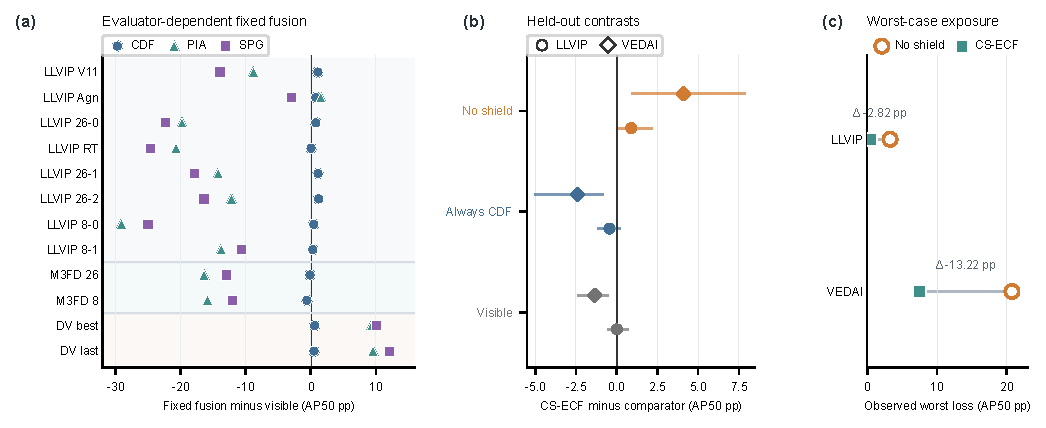
\includegraphics[width=\linewidth]{Figure3_core_evidence.pdf}
\caption{\textbf{Core evidence for detector-conditioned arbitration.}
(\textbf{a}), Fixed CDF, PIAFusion, and SPGFusion differences from visible
across 12 retrospective checkpoints directly show evaluator-dependent sign
changes. Abbreviations are expanded in the source data. (\textbf{b}), Held-out
LLVIP and VEDAI comparisons with standard confidence-ordered matching.
(\textbf{c}), Observed worst-loss reduction of CS-ECF relative to no shield.
Panel (a) is descriptive and uses the study's maximum-cardinality protocol;
panels (b,c) use standard matching and conditional resampling intervals.
Source data are provided in \texttt{Figure3\_source.csv}.}
\label{fig:core}
\end{figure}

\subsection{Budgeted candidate-library selection}

At the frozen \(K=5\) and margin \(1.5\), the development-feasible minimum
subset was visible plus PIAFusion. Its mean development gain was
\(+0.00206\), its worst evaluator gain was \(+0.00039\), and all four
evaluator cells were positive. The four-candidate policy had a lower
development mean of \(+0.00085\), one negative evaluator, and a worst gain of
\(-0.00007\). The selected subset therefore eliminated SPGFusion and CDF
without losing validation performance.

On the standard-matched LLVIP holdout, the selected subset gained
\(+0.00337\) \([-0.00016,+0.01267]\) AP50 over visible input, with five of six
positive checkpoints and a worst-checkpoint loss of \(0.00043\). Relative to
no-shield selection, the gain was \(+0.01218\) \([+0.00136,+0.02915]\), with all
six checkpoints positive. Relative to the full four-candidate CS-ECF policy,
the observed mean difference was \(+0.00325\)
\([-0.00026,+0.01051]\). Its AP50--95 contrast versus visible was
\(+0.00221\) \([-0.00006,+0.00788]\), with six of six positive checkpoints.
These intervals remain conditional on the observed scene, checkpoint, and
block hierarchy.

\DIFaddbegin \DIFadd{Because that evaluation followed subset selection, we recorded a new temporal
protocol before scoring LLVIP sequences 080, 090, and 100. The fixed sample
contains 300 non-empty frames per sequence. The policy and margin were
unchanged. It gained \(+0.01560\) \([+0.00249,+0.02874]\) AP50 over visible,
with positive equal-sequence gains of \(+0.02543\), \(+0.01924\), and
\(+0.00213\), and positive gains on all six checkpoints. The worst checkpoint
gained \(+0.00784\). The AP50--95 contrast was \(+0.00946\)
\([+0.00113,+0.01769]\).
}

\DIFadd{The gate, rather than PIAFusion itself, produced this result. Always using
PIAFusion had an equal-sequence AP50 change of \(-0.01237\)
\([-0.15111,+0.07787]\). Its sequence values were \(+0.05415\), \(+0.06766\),
and \(-0.15891\). The frozen rule switched \(5.22\%\) of image-checkpoint
cases, tied on \(95.20\%\), won on \(4.22\%\), and lost on \(0.57\%\). The gain
is therefore concentrated in the images that pass the confidence margin.
This temporal confirmation does not remove the negative VEDAI and
DroneVehicle results.
}

\DIFaddend The external boundary was not removed. The same frozen two-candidate policy
was \(-0.00329\) \([-0.00884,+0.00011]\) AP50 relative to visible on VEDAI and
\(-0.00124\) \([-0.00578,+0.00280]\) on the two independent DroneVehicle runs.
It remained better than no-shield selection on average in both domains
(\(+0.05131\) and \(+0.00421\)), but not relative to visible. Across the three
external evaluators the visible-relative difference was \(+0.01844\)
\([+0.00187,+0.03871]\); this is descriptive because those evaluators differ
in training modality and the interval spans only seven scenes. The selected
subset thus reduces the cost of a validated policy. It is not a universal
accuracy gain, and a failed target-domain validation returns visible input.

\begin{figure}[H]
\centering
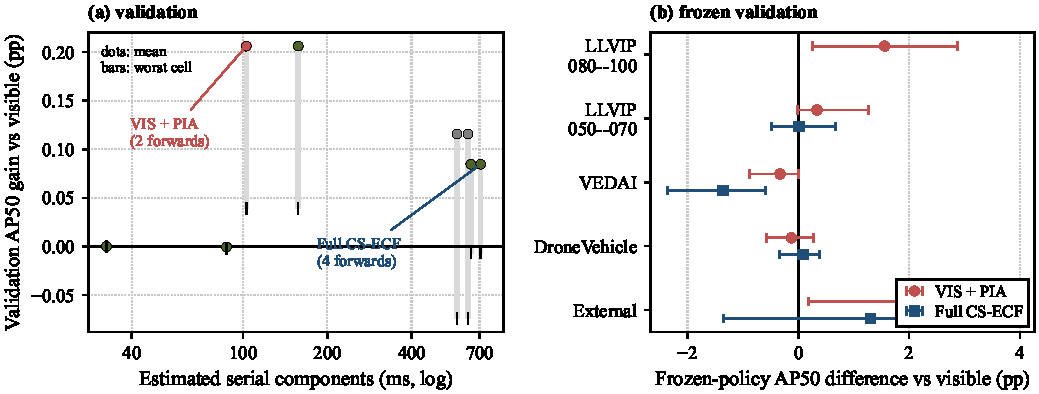
\includegraphics[width=\linewidth]{FigureBudgetedSelection.pdf}
\caption{\textbf{Budgeted candidate-library selection and transfer boundary.}
(\textbf{a}), Development evaluator mean and worst-cell AP50 gain at the
fixed \(K=5\), margin \(1.5\) policy. Each point is a candidate subset; the
horizontal position is the estimated serial component cost. The filled red
point is the selected visible plus PIAFusion subset. (\textbf{b}), Frozen
policy evaluated against visible input\DIFdelbeginFL \DIFdelFL{on standard-matched }\DIFdelendFL \DIFaddbeginFL \DIFaddFL{. The first row is the later }\DIFaddendFL LLVIP
\DIFaddbeginFL \DIFaddFL{temporal confirmation; subsequent rows are earlier LLVIP 050--070}\DIFaddendFL , VEDAI,
independent DroneVehicle\DIFdelbeginFL \DIFdelFL{runs}\DIFdelendFL , and \DIFaddbeginFL \DIFaddFL{external-evaluator tests. Only }\DIFaddendFL the \DIFdelbeginFL \DIFdelFL{three external evaluators}\DIFdelendFL \DIFaddbeginFL \DIFaddFL{selected
policy was rescored in the new temporal holdout}\DIFaddendFL . Symbols are equal-sequence or
equal-run means and intervals are conditional resampling summaries. \DIFdelbeginFL \DIFdelFL{The selected subset was not part of the original prospective
protocol; panel (b) is }\DIFdelendFL \DIFaddbeginFL \DIFaddFL{External
domains remain }\DIFaddendFL exploratory. Source data are provided in
\texttt{FigureBudgetedSelection\_source.csv}.}
\label{fig:budgeted}
\end{figure}

\subsection{System-level joint-detection reference}

We also trained the recent YOLOv11-RGBT early-fusion detector on the same
1,600/400/200 M3FD split and 40-epoch budget
(Table~\ref{tab:joint-baseline}). This system accepts a four-channel
visible--infrared image and optimizes fusion and detection together. Because
both the representation and detector change, we use its result only to
document one reproducible end-to-end implementation. The within-checkpoint
comparisons remain the evidence for the selector. The visible baselines use a
different optimization schedule, the joint model is run once, and several rare
classes are poorly represented in its score. We therefore make no performance
ranking from Table~\ref{tab:joint-baseline}.

\begin{table}[t]
\centering
\small
\caption{System-level M3FD comparison. The visible-trained rows use the same
held-out test groups and the study AP protocol. YOLOv11-RGBT jointly trains
four-channel fusion and detection and is not an architecture-matched
comparator. Its single-seed, resize-only pilot is not an estimate of best
attainable performance or evidence of intrinsic framework inferiority. Source
data are provided in
\texttt{TableJointBaseline\_source.csv}.}
\label{tab:joint-baseline}
\begin{tabular}{@{}llc@{}}
\toprule
System & Input setting & AP50 \\
\midrule
YOLO26n & visible-only checkpoint & 0.3717 \\
YOLO26n & CS-ECF on the same checkpoint & 0.3757 \\
YOLOv8n & visible-only checkpoint & 0.3790 \\
YOLOv8n & CS-ECF on the same checkpoint & 0.3972 \\
YOLOv11-RGBT & joint four-channel fusion and detection & 0.0963 \\
\bottomrule
\end{tabular}
\end{table}

The pooled AP50 entries in Table~\ref{tab:joint-baseline} are not the paired
estimand. On the two M3FD held-out frame groups, the equal-group
CS-ECF-minus-visible differences were \(+0.00291\) \([0.00000,+0.00582]\) for
YOLO26n and \(+0.01281\) \([0.00000,+0.02561]\) for YOLOv8n. Both intervals
are conditional on only two frame groups. Each evaluator in that archive
represented one training run. After the policy had been frozen, we trained
seeds 1 and 2 for both families with the same 40-epoch recipe and jointly
rescored all six checkpoints against the four candidates. The CS-ECF gain over
visible input was positive in all 6 of 6 runs. Its pooled mean was \(+0.00852\)
(range \(+0.00179\) to \(+0.01809\)), and its equal-group mean was \(+0.00617\)
(range \(+0.00175\) to \(+0.01278\)). The variation across seeds was
substantial, but every within-run contrast remained positive. The six runs
still represent two model families and only two held-out frame groups. Absolute
AP50 values in this jointly rescored archive are therefore compared only within
run and not with earlier archive values. These results strengthen the observed
within-run direction without creating cross-domain confirmation.
Run-level values and source data are provided in the Supplementary Material.

\subsection{Portability and mechanism boundaries}

The frozen selector also operated on three external detector checkpoints.
Both zero-shot evaluators improved on visible input, but no-shield selection
exceeded CS-ECF on both. The equal-scene CS-ECF-minus-no-shield contrasts were
\(-0.0179\) and \(-0.0098\), with intervals crossing zero. An LLVIP-trained
YOLOv9t reversed the visible-relative contrast, with a change of \(-0.0142\);
CS-ECF exceeded no shield there but still remained below visible. Thus neither
the visible-relative gain nor the shield-versus-no-shield ordering transferred
across all checkpoints (Fig.~\ref{fig:external}).

The matched image-statistic audit did not produce a usable operating point at
the CS-ECF switching budget, so the study does not establish a
confidence-specific mechanism. This limitation is part of the result rather
than a claim to be inferred away. Detailed control, calibration, class, and
thermal analyses are retained in the Supplementary Material.

\begin{figure}[H]
\centering
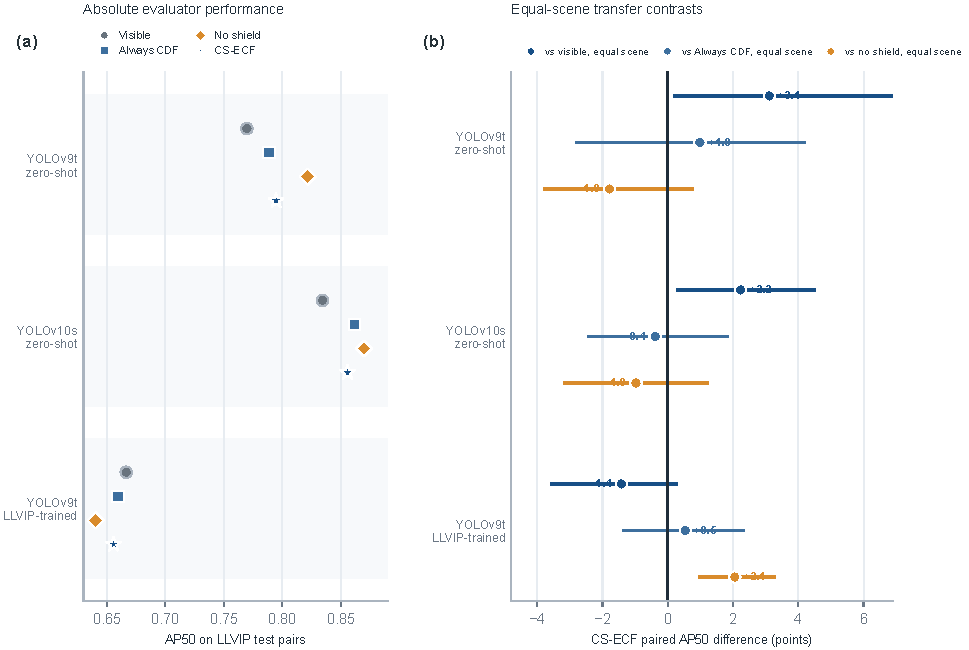
\includegraphics[width=0.90\linewidth]{Figure7_external_evaluators.pdf}
\caption{\textbf{External-evaluator portability stress tests.} Zero-shot
detectors support a visible-relative gain but not CDF superiority, and their
no-shield point estimates exceed CS-ECF. The LLVIP-trained checkpoint reverses
the visible-relative sign while CS-ECF exceeds no shield. Intervals are
descriptive and conditional on seven scene groups. Source data are provided in
\texttt{Figure7\_source.csv}.}
\label{fig:external}
\end{figure}

\subsection{Successful and failed switches}

The selected-case audit illustrates both ends of the decision problem. The
YOLO26n seed-0 checkpoint switched 17 of 1,395 images: 8 improved, 5 degraded,
and 4 were unchanged. For Fig.~\ref{fig:cases}, we selected cases whose matched
true-positive count changed. In the success case, visible input missed the
single annotated pedestrian in sequence frame 070142. SPGFusion produced a true
positive at confidence 0.67 and raised per-image AP50 from 0 to 1. In the failure case,
visible input in frame 070162 matched two of three pedestrians, whereas
SPGFusion retained only one. The examples are illustrative endpoints selected by a fixed rule, not
estimates of the average effect.

\begin{figure}[H]
\centering
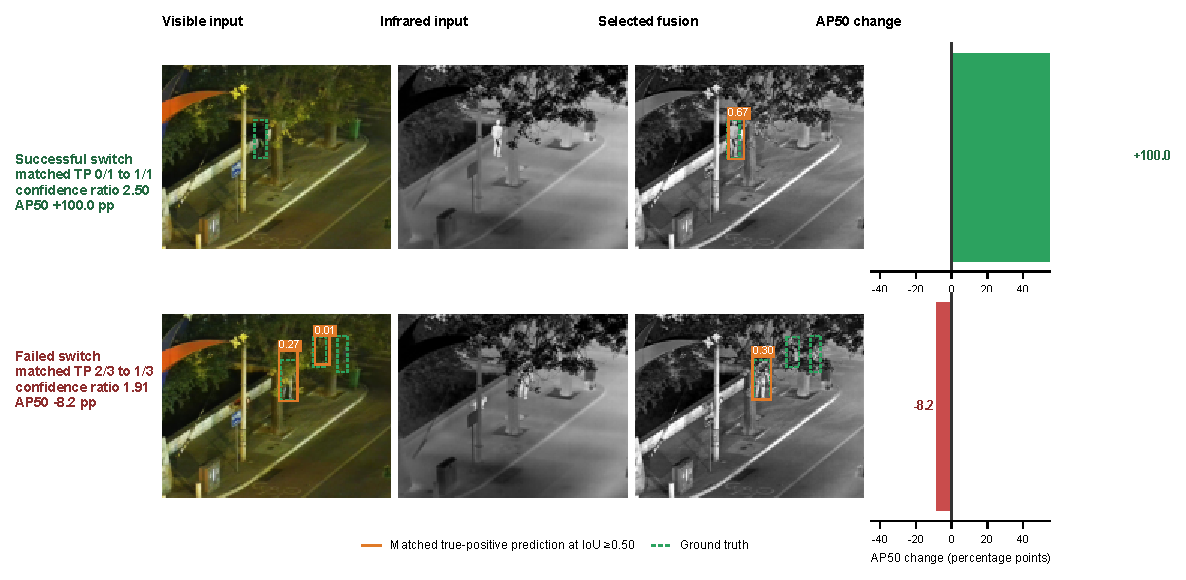
\includegraphics[width=0.96\linewidth]{Figure6_case_studies.pdf}
\caption{\textbf{Successful and failed CS-ECF switches.} The two rows show a
successful and a failed switch from the YOLO26n seed-0 checkpoint over LLVIP
sequences 050, 060, and 070. The examples are frames 070142 and 070162. Cases
were selected by a fixed rule requiring a
change in matched true-positive count that remains visible to a reader. Each
row shows visible input, infrared input, the selected fusion image, and the
paired AP50 change. Solid boxes are matched true-positive predictions at an
IoU of 0.50, annotated with detector confidence; dashed boxes are ground truth.
Ground truth is used only for this explanatory visualization, not for policy
selection. The examples are selected endpoints, not average effects. Source
data are provided in
\texttt{Figure6\_source.csv}.}
\label{fig:cases}
\end{figure}

\subsection{Operational interpretation}

The operational rule is stricter than a minimum-margin rule alone. First, use
visible input when a fused subset fails the development loss bound. Otherwise,
select the smallest feasible candidate subset rather than defaulting to the
full library. Before deployment, reproduce the matched-random comparison and
the candidate-subset check on representative groups for the target checkpoint
and domain. The selected subset should also retain its direction under the
decision-relevant metric and fit the latency and memory budget. A
switching-rate reduction alone, a full-library validation result, or a
development gain in another domain is insufficient. These are validation
gates, not measured operating guarantees (Fig.~\ref{fig:cost}).

\begin{figure}[H]
\centering
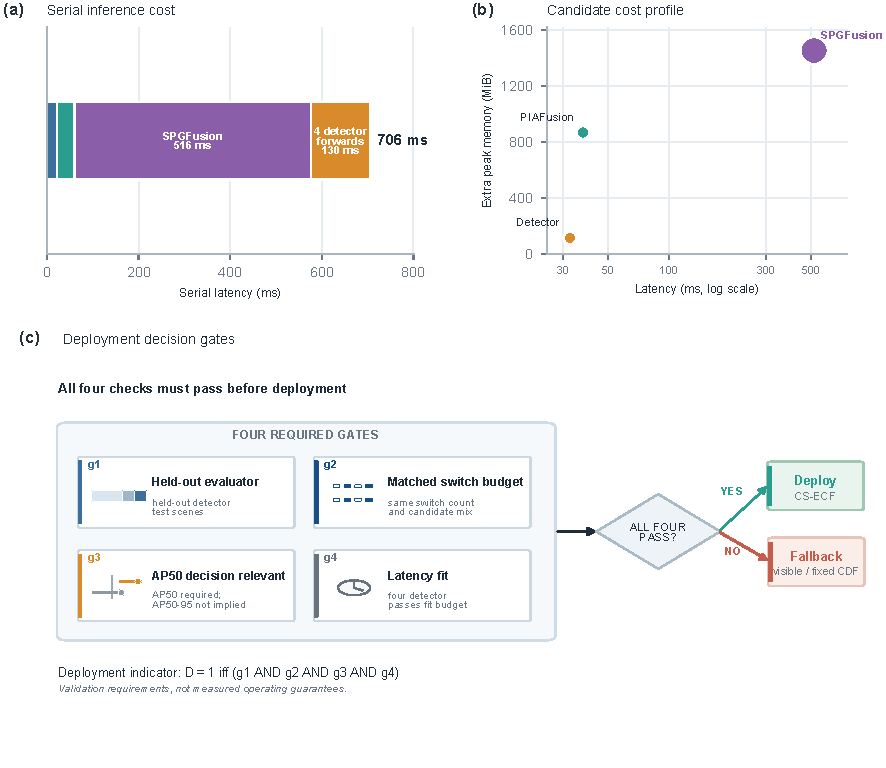
\includegraphics[width=\linewidth]{Figure11_cost_deployment.pdf}
\caption{\textbf{Cost and deployment boundaries.} Component timing,
non-additive peak memory, and four validation gates required before choosing
CS-ECF. A failed gate returns the system to visible input or stable fixed CDF.
The figure does not define a validated deployment threshold or a latency
guarantee. Source data are provided in
\texttt{Figure11\_source.csv}.}
\label{fig:cost}
\end{figure}


\section{Discussion}

The principal finding is that fusion utility is not an intrinsic property of a
fused image. The fixed-candidate matrix shows the CDF, PIAFusion, and SPGFusion
contrasts changing in magnitude or sign across detectors and domains. A policy
that selects the strongest detector response without an additional margin also
accumulated a larger observed AP50 downside. CS-ECF addresses this specific
problem by requiring a large visible-relative confidence margin before it
departs from the visible fallback. The budgeted candidate-library analysis adds
a second decision: a fused candidate should be evaluated only if the target
detector requires it. At the frozen score and margin, visible plus PIAFusion
was the smallest development-feasible subset\DIFdelbegin \DIFdel{and reduced the estimated serial
component cost from 706.3 to 102.7 ms}\DIFdelend \DIFaddbegin \DIFadd{. On a later 900-frame LLVIP
holdout, the frozen two-candidate policy gained \(+0.01560\) AP50 and
\(+0.00946\) AP50--95 over visible input, with positive results across all
three sequences and six checkpoints}\DIFaddend .

The held-out evidence supports a narrow AP50 risk-control role rather than a
general accuracy gain. Standard confidence-ordered matching preserved the
qualitative result for the full library: CS-ECF did not exceed visible input,
remained below fixed CDF, and exceeded no-shield selection by \(+0.00894\) on
LLVIP. A random control matched to the same switching count and candidate mix
showed a \(+0.01392\) deficit, so the AP50 result is not explained by switch
frequency alone. The selected two-candidate policy had a larger descriptive
mean than the full library \DIFaddbegin \DIFadd{in the earlier LLVIP evaluation }\DIFaddend and a positive
no-shield contrast\DIFdelbegin \DIFdel{, but its
visible-relative interval crossed zero. It also }\DIFdelend \DIFaddbegin \DIFadd{. Its later temporal holdout was also positive. Ungated
PIAFusion nevertheless lost \(0.15891\) AP50 on the third confirmation
sequence, showing why the confidence gate remains necessary. The policy still
}\DIFaddend failed to improve on visible \DIFdelbegin \DIFdel{on }\DIFdelend \DIFaddbegin \DIFadd{in }\DIFaddend VEDAI and the independent DroneVehicle runs.
Candidate-library reduction is therefore a compute decision made after
target-specific validation, not a replacement for that validation.

We additionally document a same-split YOLOv11-RGBT system-level pilot. Because
its fusion representation and detector are optimized together,
its score cannot isolate the effect of fusion selection. The single-seed,
resize-only run has different optimization and rare-class conditions from the
visible comparators. We therefore use it only as an implementation pilot,
while the claims about CS-ECF remain based on within-checkpoint comparisons
against visible, Always CDF, and no shield.

Mechanistic and portability claims are therefore limited. Matched
image-statistic controls did not provide a usable operating point. Two
zero-shot evaluators reversed the no-shield ordering, while an LLVIP-trained
evaluator reversed the visible-relative sign. These observations may reflect
calibration, train-to-test shift, or other checkpoint-specific differences;
the present design does not separate those explanations. CDF is study-internal,
so the selector and this particular fusion construction should not be treated
as separable published-method effects.

For operation, visible input should remain the default. A candidate subset and
confidence margin are justified only after target-checkpoint and
target-domain validation, a switch-budget-matched comparison, and confirmation
that AP50 is the decision-relevant endpoint. The smallest feasible subset
should then be selected under the measured latency and memory budget. If no
fused subset passes the development constraint, or if the selected subset
fails target-domain validation, the procedure returns visible input. The
\DIFdelbegin \DIFdel{reported 102.7 ms and 706.3 ms values are component measurements, not end-to-end deployment guarantees}\DIFdelend \DIFaddbegin \DIFadd{measured end-to-end medians were 1.67 s for the selected pipeline and 2.52 s
for the full library. The selected pipeline reduces cost by one third but does
not satisfy a low-latency deployment claim}\DIFaddend .

\subsection*{Limitations}

The \DIFdelbegin \DIFdel{candidate-library result is exploratory because the original prospective
protocol fixed the full library, and the }\DIFdelend two-candidate subset was selected during revision\DIFdelbegin \DIFdel{. The }\DIFdelend \DIFaddbegin \DIFadd{, outside the original
prospective protocol. Its later confirmation uses three new sequences and 900
frames selected by a resource amendment recorded before scoring. The interval
is conditional on those three sequences and six fixed runs. The }\DIFaddend development
split is image-disjoint but not scene-group-disjoint for LLVIP. DroneVehicle
contributes two independent runs, M3FD contributes two held-out frame groups\DIFdelbegin \DIFdel{and one training run per evaluator}\DIFdelend ,
and the external-evaluator interval spans seven scene groups. These designs
quantify observed heterogeneity but do not estimate \DIFdelbegin \DIFdel{a }\DIFdelend population-level coverage\DIFdelbegin \DIFdel{guarantee}\DIFdelend .
The full policy did not preserve its AP50--95 direction, and matched
image-statistic controls did not identify a mechanism. The YOLOv11-RGBT
comparison changes representation and detector together and remains a
single-seed implementation pilot. CDF is a study-internal construction rather
than a published fixed baseline.

\section{Conclusions}

We evaluated CS-ECF as a detector-conditioned AP50 safeguard against harmful
fusion-input switching. Scene-disjoint LLVIP and VEDAI tests both favored the
shield over unconstrained selection under standard confidence-ordered matching,
and a switch-budget-matched random control was worse. The same experiments did
not establish a visible-relative gain or superiority over Always CDF. External
evaluators reversed the no-shield ordering, and the advantage did not persist
under AP50--95. Matched controls also did not isolate a confidence-specific
mechanism. The YOLOv11-RGBT run is a single-seed implementation pilot rather
than a performance ranking.

The candidate-library analysis further shows that the full four-candidate
library is not required for every validated deployment. At the frozen score
and margin, visible plus PIAFusion was the smallest development-feasible
subset\DIFdelbegin \DIFdel{and reduced the component estimate from 706.3 to 102.7 ms. Its larger
LLVIP mean }\DIFdelend \DIFaddbegin \DIFadd{. On the new 900-frame LLVIP holdout it improved AP50 and AP50--95, but
ungated PIAFusion reversed sharply on one sequence. The policy }\DIFaddend did not transfer
to VEDAI or the independent DroneVehicle runs\DIFaddbegin \DIFadd{. Its measured end-to-end median
was \(1.67\) s versus \(2.52\) s for the full library, so the subset reduces
but does not eliminate deployment cost}\DIFaddend .

The practical conclusion is therefore conditional on both the target
evaluator and the deployment domain. Visible fallback should remain the
default. A detector-specific validation should first decide whether any fused
subset is justified, then choose the smallest feasible subset, verify a
switch-budget-matched comparison and AP50 endpoint, and fall back to visible
when those checks fail.

\section*{CRediT authorship contribution statement}

\textbf{Jianyong Zhao:} Conceptualization, Methodology, Software, Formal
analysis, Writing -- original draft. \textbf{Zigao Wu:} Supervision, Writing
-- review \& editing. \textbf{Mengfei Ma:} Investigation, Validation,
Writing -- review \& editing.

\section*{Declaration of competing interest}

The authors declare that they have no known competing financial interests or
personal relationships that could have appeared to influence the work reported
in this article.

\section*{Funding}

This research did not receive any specific grant from funding agencies in the
public, commercial, or not-for-profit sectors.

\section*{Data availability}

The underlying datasets are publicly available. LLVIP is distributed at
\url{https://github.com/bupt-ai-cz/LLVIP}. M3FD is distributed with the TarDAL
benchmark at \url{https://github.com/JinyuanLiu-CV/TarDAL}. DroneVehicle is
distributed through \url{https://github.com/VisDrone/DroneVehicle} and was
obtained from the public archive
\url{https://huggingface.co/datasets/McCheng/DroneVehicle}. VEDAI is available
from \url{https://downloads.greyc.fr/vedai/} for non-commercial research use
under the provider's terms. Each dataset is used under the license stated by
its distributor. The public analysis repository provides fixed train,
validation, and test manifests for LLVIP, M3FD, DroneVehicle, and VEDAI;
source-archive metadata; per-image CS-ECF scores; standard-matching and
switch-matched controls; and the hashed prospective LLVIP protocol. It also
includes LLVIP sequence 040--070 score arrays, native DroneVehicle OBB scores,
independent-run manifests, and source-data tables. Scripts regenerate the
reported equal-group and prospective intervals.

\section*{Code availability}

The code for reproducing the experiments is available at
\url{https://github.com/lessThanbetter/ssgf} under an MIT license. The
project-level record is available under the concept DOI
\url{https://doi.org/10.5281/zenodo.22984388}. The repository contains the
fusion and arbitration code, detector-evaluation scripts, fixed split and test
manifests, the prospective protocol, and a native OBB scoring adapter. It also
includes independent DroneVehicle training code, VEDAI fold preparation and
training/scoring code, and per-image scores. The submission archive and
\texttt{SHA256SUMS.txt} identify the exact files used for this analysis. They
also include result tables, figure source data, a figure-number mapping, and
numerical checks used to generate the reported intervals.

\section*{Declaration of generative AI and AI-assisted technologies in the
manuscript preparation process}

During the preparation of this manuscript, the authors used an AI-assisted
writing tool solely to improve language, clarity, and readability. No AI was
used for data collection, experimental work, data analysis, model training,
figure generation, or the interpretation of results. The authors reviewed and
edited all AI-assisted text and take full responsibility for the content of the
publication.

\begingroup
\footnotesize
\bibliographystyle{elsarticle-num}
\bibliography{references}
\endgroup

\end{document}
